% TL;DR: Projektkarte als U-Bahn-Plan (Mai–Nov. 2026), nur die Karte; Varianten (A4, Poster, Folie) binden das erzeugte PDF ein. Quelle der Zahlen: docs/ergebnisse/diagnose-chronik.md.
%
% Aufruf über build.sh. Variante über \def\kartevariante{voll|kurz} vor \input:
%   voll = alle Stationen mit Detailzeile (A4, Poster, README)
%   kurz = nur Wendepunkte und markierte Stationen, ohne Detailzeile (Folie)
\documentclass[border=2mm]{standalone}
\usepackage{libertinus-otf}
\usepackage{xcolor}
\usepackage{tikz}
% TL;DR: Gemeinsame Farben, TikZ-Stile und Stations-Makros der Projektkarte (U-Bahn-Plan); wird von karte.tex und den Varianten eingebunden.
%
% Lesart der Karte
%   Linie       = Arbeitsstrang (Farbe)
%   Station     = Meilenstein; die Füllung zeigt den Ausgang (\Mk)
%   Stumpfgleis = aufgegebener Weg (endet mit Prellbock)
%   Fehlannahme = gestrichelte Nebenspur (Stil irrweg): so lange galt eine falsche Annahme

\usetikzlibrary{positioning, calc, patterns, shapes.geometric, fit, backgrounds, arrows.meta}

% ── Linienfarben (Arbeitsstränge) ─────────────────────────────────────
\definecolor{lInfra}{HTML}{6B7B8C}   % Infrastruktur / Rechenzugang
\definecolor{lTrain}{HTML}{1F4E9C}   % Training N1.6 (NavyBlue wie die Ausarbeitung)
\definecolor{lNsieben}{HTML}{8E44AD} % GR00T N1.7
\definecolor{lCotr}{HTML}{D1477A}    % Co-Training / Daten
\definecolor{lSim}{HTML}{0E8C7F}     % Simulation / Szene
\definecolor{lDiag}{HTML}{E07B00}    % Evaluation / Diagnose
\definecolor{lRL}{HTML}{8D8D8D}      % Reinforcement Learning
\definecolor{lDoku}{HTML}{3C3C3C}    % Doku / Abgabe

% ── Statusfarben (Stationen) ──────────────────────────────────────────
\definecolor{sOk}{HTML}{2E8B3E}      % Erfolg
\definecolor{sFail}{HTML}{C62828}    % Fehlschlag
\definecolor{sPart}{HTML}{F2B705}    % Teilerfolg
\definecolor{sOld}{HTML}{9E9E9E}     % verworfen / überholt
\definecolor{phaseA}{HTML}{F4F6F9}
\definecolor{phaseB}{HTML}{E9EDF3}
\definecolor{hubbg}{HTML}{FFF8E1}

% ── Maße (die Varianten skalieren die fertige Karte als Ganzes) ───────
\newcommand\linew{2.6pt}
\newcommand\fsLbl{\fontsize{6.4}{7.3}\selectfont\sffamily}
\newcommand\fsPhase{\fontsize{7.2}{8.4}\selectfont\sffamily}

\tikzset{
  line/.style   = {line width=\linew, line cap=round, line join=round, rounded corners=4mm},
  stub/.style   = {line width=\linew, line cap=butt, dash pattern=on 3pt off 2pt},
  irrweg/.style = {line width=1.1pt, dash pattern=on 2.4pt off 1.6pt, line cap=round,
                   rounded corners=2.5mm},
  lbl/.style    = {font=\fsLbl, align=center, inner sep=0.6pt, text depth=0pt},
  badge/.style  = {rounded corners=1.6mm, font=\fontsize{6.8}{7.6}\selectfont\sffamily\bfseries,
                   text=white, inner xsep=1.6mm, inner ysep=1.1mm, minimum width=19mm,
                   align=center},
}

% \Mk{status}{x,y}: Stationsmarke. status ∈ ok | fail | part | old | open
\newcommand\Mk[2]{%
  \begin{scope}[shift={(#2)}]
    \fill[white] (0,0) circle (1.95mm);
    \csname mk@#1\endcsname
  \end{scope}}
\makeatletter
\newcommand\mk@ok{\fill[sOk] (0,0) circle (1.45mm);
  \draw[white, line width=0.85pt, line cap=round, line join=round]
    (-0.72mm,0.02mm) -- (-0.18mm,-0.58mm) -- (0.78mm,0.62mm);}
\newcommand\mk@fail{\fill[sFail] (0,0) circle (1.45mm);
  \draw[white, line width=0.85pt, line cap=round]
    (-0.6mm,-0.6mm) -- (0.6mm,0.6mm) (-0.6mm,0.6mm) -- (0.6mm,-0.6mm);}
\newcommand\mk@part{\fill[white] (0,0) circle (1.45mm);
  \fill[sPart] (0,-1.45mm) arc (-90:90:1.45mm) -- cycle;
  \draw[sPart!80!black, line width=0.6pt] (0,0) circle (1.2mm);}
\newcommand\mk@old{\fill[sOld] (0,0) circle (1.45mm);
  \draw[white, line width=0.8pt] (-0.75mm,0) -- (0.75mm,0);}
\newcommand\mk@open{\fill[white] (0,0) circle (1.45mm);
  \draw[black!70, line width=0.6pt, dash pattern=on 0.9pt off 0.7pt] (0,0) circle (1.2mm);}
\makeatother

% \Wende{x,y}: Wendepunkt (schwarzer Ring um die Station)
\newcommand\Wende[1]{\draw[black, line width=0.9pt, fill=white] (#1) circle (2.55mm);}

% \St[*]{status}{x}{y}{Platzierung}{Titel}{Detail}
%   *            = Wendepunkt
%   Platzierung  = above | below | left | right | above left | ... (Abstand fest)
% Abstand der Beschriftung zur Marke; Wendepunkte brauchen mehr wegen des Rings
\newcommand\lblsep{2.35mm}
\newcommand\lblsepW{3.3mm}
\NewDocumentCommand\St{s m m m m m m}{%
  \IfBooleanTF{#1}{\Wende{#3,#4}\def\sep{\lblsepW}}{\def\sep{\lblsep}}%
  \Mk{#2}{#3,#4}%
  \node[lbl, #5=\sep] at (#3,#4) {{\bfseries #6}\ifx\relax#7\relax\else\\#7\fi};}

% \Prellbock{x,y}{Winkel}: Ende eines Stumpfgleises (Querbalken)
\newcommand\Prellbock[3][black]{%
  \draw[#1, line width=1.6pt, line cap=butt] ($(#2)+(#3+90:1.7mm)$) -- ($(#2)+(#3-90:1.7mm)$);}

% \Legende: Zeichenerklärung als eigenes Bild (Varianten skalieren mit \scalebox)
\newcommand\Legende{%
\begin{tikzpicture}[x=1cm, y=1cm, every node/.style={font=\fsLbl, anchor=west, inner sep=1pt}]
  \Mk{ok}{0,0}\node at (0.25,0) {Erfolg};
  \Mk{part}{1.45,0}\node at (1.7,0) {Teilerfolg};
  \Mk{fail}{3.25,0}\node at (3.5,0) {Fehlschlag};
  \Mk{old}{5.1,0}\node at (5.35,0) {verworfen / überholt};
  \Wende{7.95,0}\Mk{ok}{7.95,0}\node at (8.25,0) {Wendepunkt};
  \draw[stub, black!70] (10.1,0) -- (10.9,0); \Prellbock[black!70]{10.9,0}{0}
  \node at (11.05,0) {Stumpfgleis = aufgegebener Weg};
  \draw[irrweg, black!70] (15.3,0) -- (16.1,0);
  \node at (16.2,0) {Fehlannahme = Dauer bis zur Widerlegung};
  \node at (20.55,0) {T$n$ = Trainingslauf $n$ · L$n$ = Diagnoselauf $n$ · Zeitachse nicht maßstäblich};
\end{tikzpicture}}

% \BlockerKette: Ursachenkette als Zeile (jede gelöste Ebene legte die nächste frei)
\newcommand\BlockerKette{%
\begin{tikzpicture}[x=1cm, y=1cm,
    bk/.style={draw=black!45, line width=0.5pt, fill=white, rounded corners=1.2mm,
      font=\fsLbl, align=center, text width=31mm, minimum height=9.5mm, inner sep=1.2pt},
    pf/.style={-{Latex[length=1.6mm]}, line width=0.9pt, black!55}]
  \node[font=\fsLbl\bfseries, anchor=east, align=right] at (-0.25,0)
    {Blocker-Kette:\\[-1pt]{\mdseries jede gelöste Ebene}\\[-1pt]{\mdseries legte die nächste frei}};
  \foreach \i/\s/\t/\d in {
      0/ok/{Kameras verdreht}/{behoben, L10–18},
      1/ok/{Geometrie: Finger, Becken, Basis}/{behoben, L38–51},
      2/part/{Würfel 3 cm versetzt}/{korrigiert, Ursache offen, L62},
      3/part/{Bild-Lücke Sim ↔ Echt}/{×13 → halbiert, L66/L83},
      4/part/{Griff}/{2/60 frei gehoben, L97},
      5/open/{Stapeln + Robotertest}/{0/60, offen}} {
    \node[bk] (b\i) at ({\i*3.75+1.75},0) {{\bfseries\t}\\\d};
    \Mk{\s}{{\i*3.75+0.12},0.47}
  }
  \foreach \i [evaluate=\i as \j using int(\i+1)] in {0,...,4} \draw[pf] (b\i.east) -- (b\j.west);
\end{tikzpicture}}


\providecommand\kartevariante{voll}
\newif\ifkurz
\def\tmpkurz{kurz}
\ifx\kartevariante\tmpkurz \kurztrue \fi

% Im Kurzmodus: Beschriftung nur für Wendepunkte (*) und Schlüsselstationen (!)
\ifkurz
  \RenewDocumentCommand\St{s t! m m m m m m}{%
    \IfBooleanT{#1}{\Wende{#4,#5}}%
    \Mk{#3}{#4,#5}%
    \IfBooleanTF{#1}{\node[lbl, #6=2.35mm] at (#4,#5) {{\bfseries #7}};}{%
      \IfBooleanT{#2}{\node[lbl, #6=2.35mm] at (#4,#5) {{\bfseries #7}};}}}
\else
  \RenewDocumentCommand\St{s t! m m m m m m}{%
    \IfBooleanT{#1}{\Wende{#4,#5}}%
    \Mk{#3}{#4,#5}%
    \node[lbl, #6=2.35mm] at (#4,#5) {{\bfseries #7}\ifx\relax#8\relax\else\\#8\fi};}
\fi
\newcommand\Detail[1]{\ifkurz\else#1\fi}
\ifkurz % Folie: größere Schrift, weniger Text
  \renewcommand\fsLbl{\fontsize{8.4}{9.4}\selectfont\sffamily}
  \renewcommand\fsPhase{\fontsize{8.4}{9.6}\selectfont\sffamily}
  \tikzset{badge/.append style={font=\fontsize{8}{8.8}\selectfont\sffamily\bfseries, minimum width=19mm, inner xsep=1mm}}
\fi

\begin{document}
\begin{tikzpicture}[x=1cm, y=1cm]

% ── Lagen der Linien (y) ──────────────────────────────────────────────
\def\yI{0}      % Infrastruktur
\def\yT{-2.0}   % Training N1.6
\def\yN{-3.35}  % N1.7
\def\yC{-5.1}   % Co-Training / Daten
\def\yS{-7.1}   % Simulation / Szene
\def\yD{-9.6}   % Evaluation / Diagnose
\def\yR{-12.3} % RL
\def\yK{-13.45} % Doku / Abgabe
\def\xH{24.0}   % linke Kante "Stand heute"

% ── Phasenbänder (Zeitachse nicht maßstäblich) ────────────────────────
\begin{scope}[on background layer]
  \foreach \xa/\xb/\cc/\nam/\dat in {
      0.0/4.8/phaseA/{Aufbau \& erste Läufe}/{08.05.–05.06.},
      4.8/6.6/white/{Pause}/{Prüfungen\\Juni–Juli},
      6.6/11.6/phaseA/{Sim auf Blackwell, Diagnose}/{01.–14.08.},
      11.6/14.8/phaseB/{Geometrie-Jagd}/{15.–26.08.},
      14.8/17.0/phaseA/{Synth-Daten \& N1.7}/{27.08.–11.10.},
      17.0/20.4/phaseB/{Nachmessen \& Registrierung}/{12.–14.10.},
      20.4/23.8/phaseA/{Co-Training v3}/{15.–29.10.}} {
    \pgfmathsetlengthmacro\tw{(\xb-\xa)*1cm-2mm}
    \fill[\cc] (\xa,2.7) rectangle (\xb,-14.05);
    \node[font=\fsPhase, align=center, text width=\tw, anchor=north]
      at ({(\xa+\xb)/2},2.62) {{\bfseries\nam}\\[-0.5pt]{\color{black!60}\dat}};
  }
  \fill[pattern=north east lines, pattern color=black!12] (4.8,1.25) rectangle (6.6,-14.05);
  \draw[black!35, line width=0.4pt] (0,1.25) -- (23.8,1.25);
\end{scope}

% ── Linien-Plaketten links ────────────────────────────────────────────
\foreach \y/\cc/\lab in {\yI/lInfra/{Infrastruktur},\yT/lTrain/{Training N1.6},
    \yN/lNsieben/{GR00T N1.7},\yC/lCotr/{Co-Training\\[-1pt]\& Daten},
    \yS/lSim/{Simulation\\[-1pt]\& Szene},\yD/lDiag/{Evaluation\\[-1pt]\& Diagnose},
    \yR/lRL/{Reinforcement\\[-1pt]Learning},\yK/lDoku/{Doku \& Abgabe}}
  \node[badge, fill=\cc] at (-1.25,\y) {\lab};

% ════════════════════════════ LINIEN ══════════════════════════════════
% Infrastruktur
\draw[line, lInfra] (-0.25,\yI) -- (\xH,\yI);
\draw[stub, lInfra] (2.3,\yI) -- (2.85,-0.55) -- (3.45,-0.55); \Prellbock[lInfra]{3.45,-0.55}{0}
\draw[stub, lInfra] (6.0,\yI) -- (6.55,-0.55) -- (7.2,-0.55); \Prellbock[lInfra]{7.2,-0.55}{0}

% Training N1.6
\draw[line, lTrain] (-0.25,\yT) -- (\xH,\yT);
\draw[stub, lTrain] (2.5,\yT) -- (3.05,-2.6) -- (3.7,-2.6); \Prellbock[lTrain]{3.7,-2.6}{0}
% Irrweg U-Kurve (14.08. → 12.10.)
\draw[irrweg, lTrain] (11.25,\yT) -- (11.7,-2.48) -- (16.95,-2.48) -- (17.25,\yT);

% N1.7 (zweigt am 19.08. ab)
\draw[line, lNsieben] (12.4,\yT) -- (13.75,\yN) -- (\xH,\yN);

% Co-Training / Daten
\draw[line, lCotr] (11.9,\yC) -- (\xH,\yC);
\draw[stub, lCotr] (12.75,\yC) -- (13.3,-5.65) -- (13.8,-5.65); \Prellbock[lCotr]{13.8,-5.65}{0}

% Simulation / Szene
\draw[line, lSim] (-0.25,\yS) -- (\xH,\yS);
% Irrweg Finger-Vorzeichen (≤ 04.06. → 24.08.)
\draw[irrweg, lSim] (3.55,\yS) -- (4.25,-8.3) -- (13.5,-8.3) -- (13.95,\yS);

% Evaluation / Diagnose
\draw[line, lDiag] (-0.25,\yD) -- (\xH,\yD);
% Irrweg SigLIP-Abstand (04.06. → 14.10.)
\draw[irrweg, lDiag] (3.3,\yD) -- (3.95,-10.95) -- (18.6,-10.95) -- (19.0,\yD);

% RL
\draw[line, lRL] (4.6,\yR) -- (8.4,\yR);
\draw[stub, lRL] (8.4,\yR) -- (\xH,\yR);

% Doku
\draw[line, lDoku, line width=1.6pt] (-0.25,\yK) -- (\xH,\yK);

% Umsteigekapsel Co-Training v3 (Training, N1.7, Daten)
\draw[black, line width=0.9pt, fill=white, rounded corners=2.4mm]
  (20.95,{\yT+0.25}) rectangle (21.45,{\yC-0.25});

% ════════════════════════════ STATIONEN ═══════════════════════════════
% Infrastruktur
\St!{ok}{0.3}{\yI}{above}{Docker + Fork}{08.05.}
\St{ok}{1.95}{\yI}{above}{KISSKI-Cluster}{4× A100}
\St{ok}{3.75}{\yI}{above}{Sim auf Miet-GPU}{vast.ai}
\St{fail}{3.45}{-0.55}{right}{Sim auf KISSKI}{\Detail{keine RT-Cores}}
\St{ok}{5.6}{\yI}{above}{Institutsserver}{Blackwell, Juli}
\St{fail}{7.2}{-0.55}{right}{Isaac Sim 5.1}{\Detail{stürzt ab}}
\St*{ok}{7.6}{\yI}{above}{Isaac Sim 6.0}{08.08.}
\St{ok}{12.4}{\yI}{above}{./run.sh-Menüs}{20.08.}
\St{ok}{15.6}{\yI}{above}{Image je Generation}{29.09.}
\St{ok}{18.4}{\yI}{above}{CI + Reviews}{13.10.}
\St{part}{22.4}{\yI}{above}{Watchdog}{Hänger, Ursache offen}

% Training N1.6
\St!{ok}{1.6}{\yT}{above}{Lauf 1}{175k Schritte, Encoder fest}
\St{fail}{3.7}{-2.6}{right}{Lauf 2: Encoder trainiert}{\Detail{Policy kollabiert}}
\St{ok}{9.65}{\yT}{above}{Split aktiv}{13.08.}
\St*{ok}{11.25}{\yT}{above}{Lauf 3}{Vision + Jitter + Split}
\node[lbl, lTrain, font=\fsLbl\itshape] at (15.35,-2.74) {Irrweg: U-Kurve, »Optimum @30k«};
\St*{ok}{17.25}{\yT}{above}{Nachmessung 20×750}{@44\,000 am besten}
\St{part}{22.7}{\yT}{above}{N1.6 cube4 @44k}{greift 2/60, stapelt 0}

% N1.7
\St!{ok}{14.25}{\yN}{below}{N1.7-Pfad}{19.08.}
\St{ok}{17.25}{\yN}{below}{Lauf 4 (N1.7)}{gleichauf, 1,6× schneller}
\St{fail}{19.2}{\yN}{above}{N1.7 in der Sim}{hebt 0/10 (L54/55)}
\St{part}{22.7}{\yN}{above}{N1.7 co-trainiert}{greift 0/20}

% Co-Training / Daten
\St{old}{12.2}{\yC}{above}{Render v1}{Greifpunkt verworfen}
\St{part}{13.8}{-5.65}{right}{Cosmos-Transfer}{\Detail{nie Ende-zu-Ende}}
\St{fail}{15.1}{\yC}{above}{cotrain\_synth\_v1}{kein Co-Training}
\St{part}{17.15}{\yC}{below}{Fremd-Synthdaten}{Finger vertauscht}
\St{ok}{19.7}{\yC}{above}{Render-Daten v3}{187 Ep. (L72)}
\Mk{ok}{21.2,\yT}\Mk{ok}{21.2,\yN}\Mk{ok}{21.2,\yC}
\node[lbl, below=3.2mm] at (21.2,\yC) {{\bfseries Co-Training v3}\Detail{\\4× 44k (L73–76)}};
\St*{ok}{22.7}{\yC}{above}{Lücke halbiert}{MSE 0,024→0,012}

% Simulation / Szene
\St!{ok}{1.6}{\yS}{above}{G1 + DEX3}{in Isaac Lab}
\node[lbl, lSim, font=\fsLbl\itshape] at (6.45,-8.07) {Irrweg: Finger-Vorzeichen – Hand schließt nie};
\St{ok}{8.2}{\yS}{above}{Würfel fallen}{Offset (L8/9)}
\St*{ok}{9.6}{\yS}{below}{Kameras verdreht}{96–137° (L10–18)}
\St{part}{11.0}{\yS}{above}{Greifphysik}{hebt 7,9 cm (L29)}
\St*{ok}{13.95}{\yS}{above}{Geometrie-Jagd}{Finger, Becken, Basis}
\St*{ok}{18.3}{\yS}{above}{Würfel 3 cm innen}{Orakel 0→48\,\% (L62)}
\St{part}{20.0}{\yS}{below}{Szene ans Echtbild}{Handfehler −40\,\%}

% Evaluation / Diagnose
\St!{fail}{1.8}{\yD}{above}{Erste Sim-Eval}{Lauf 1: 0/20}
\St{old}{3.95}{-10.95}{left}{SigLIP-Gap}{0,26 / 0,43}
\node[lbl, lDiag, font=\fsLbl\itshape] at (11.3,-11.22) {Irrweg: SigLIP-Abstand als Maß der Lücke (0,22 sah »gut« aus)};
\St*{ok}{6.0}{\yD}{above}{RoboCasa-Referenz}{47,7\,\% ≈ 47,8\,\%}
\St{fail}{8.4}{\yD}{above}{Messpunkt 3× falsch}{(L24–28)}
\St*{ok}{9.8}{\yD}{below}{span-Gate}{Echt 100\,\%, Sim 19\,\%}
\St{part}{11.3}{\yD}{above}{Lauf 3 im Closed Loop}{0/10 (L34)}
\St*{fail}{16.9}{\yD}{above}{Orakel-Replay}{hebt 1/16 (L57)}
\St*{ok}{19.0}{\yD}{above}{Bild-Ablation}{Fehler ×13 / ×36}
\St{ok}{20.6}{\yD}{above}{Gate geseedet}{(L80)}
\St*{ok}{21.85}{\yD}{below}{Vorregistr. Gate}{p = 5·10⁻⁶ (L96)}
\St{part}{23.1}{\yD}{above}{60 Testlagen}{2/60 (L97)}

% RL
\St!{ok}{5.0}{\yR}{above}{RL-Plan (FPO)}{12.06.}
\St{part}{8.0}{\yR}{below}{RL-Pipeline läuft}{ohne Lerneffekt}
\node[lbl, lRL!80!black, font=\fsLbl\itshape, above=1.2mm] at (18.5,\yR)
  {wartet auf ein Griffsignal (erstmals 2/60)};

% Doku
\St{ok}{0.35}{\yK}{above}{README}{}
\St{ok}{12.6}{\yK}{above}{Doku neu geordnet}{18.08.}
\St{ok}{17.6}{\yK}{above}{Ausarbeitung neu}{11.10.}
\St!{ok}{22.6}{\yK}{above}{Abgabe-Review}{30.10.}

% ════════════════════════════ STAND HEUTE ═════════════════════════════
\begin{scope}[shift={(\xH,0)}]
  \draw[black, line width=1.2pt, fill=hubbg, rounded corners=3mm] (0,1.25) rectangle (2.75,-14.05);
  \node[font=\fontsize{9}{10}\selectfont\sffamily\bfseries, anchor=north] at (1.375,1.1) {Stand heute};
  \node[font=\fsLbl, anchor=north, black!65] at (1.375,0.6) {01.11.2026};
  % Einmündungen
  \foreach \y/\cc in {\yI/lInfra,\yT/lTrain,\yN/lNsieben,\yC/lCotr,\yS/lSim,\yD/lDiag,\yK/lDoku}
    \fill[\cc] (0,\y) circle (1.3mm);
  \node[font=\fsLbl, text width=24.5mm, align=left, anchor=north west] at (0.15,-0.35) {%
    \ifkurz {\bfseries Bestes Modell}\\N1.6 @44k\\[3pt]{\bfseries Sim-Kandidat}\\co-trainiert
    \else {\bfseries Bestes Modell}\\N1.6 vision-v2 @44k\\Val-MSE 0,00482\\[2pt]
    {\bfseries Bester Sim-Kandidat}\\N1.6 co-trainiert,\\cube4 @44k (L74)\fi};
  % Trichter Closed Loop (L97, 60 Testlagen)
  \node[font=\fsLbl\bfseries, anchor=west] at (0.18,-3.95) {Closed Loop (L97)};
  \foreach \i/\lab/\k/\n in {0/erreicht/58/60, 1/berührt/60/60, 2/gehoben/6/60,
      3/frei gehoben/2/60, 4/gestapelt/0/60} {
    \pgfmathsetmacro\w{2.35*\k/\n}
    \fill[black!10] (0.2,{-4.45-\i*0.62}) rectangle (2.55,{-4.68-\i*0.62});
    \ifnum\k>0 \fill[lDiag] (0.2,{-4.45-\i*0.62}) rectangle ({0.2+\w},{-4.68-\i*0.62}); \fi
    \node[font=\fsLbl, anchor=south west, inner sep=0.5pt] at (0.18,{-4.43-\i*0.62}) {\lab};
    \node[font=\fsLbl\bfseries, anchor=south east, inner sep=0.5pt] at (2.57,{-4.43-\i*0.62}) {\k/\n};
  }
  \node[font=\fsLbl, text width=24.5mm, align=left, anchor=north west] at (0.15,-7.65) {%
    \ifkurz
    {\bfseries Blocker}\\
    {\color{sPart!70!black}\textbullet} Würfel versetzt\\
    {\color{sPart!70!black}\textbullet} Bild-Lücke\\[4pt]
    {\bfseries Offen}\\
    {\color{sFail}\textbullet} Stapeln: 0\\
    {\color{sFail}\textbullet} kein Robotertest
    \else
    {\bfseries Zwei Blocker}\\
    {\color{sPart!70!black}\textbullet} Würfel 3 cm versetzt\\
    \hphantom{\textbullet} Orakel 6/20 (L69)\\
    {\color{sPart!70!black}\textbullet} Bild-Lücke ×13\\
    \hphantom{\textbullet} halbiert, nicht weg\\[3pt]
    {\bfseries Offen}\\
    {\color{sFail}\textbullet} gestapelt: 0\\
    {\color{sFail}\textbullet} kein Robotertest\\
    {\color{black!50}\textbullet} RL ohne Ergebnis\\[3pt]
    {\bfseries Nächster Schritt}\\
    mehr Render-Episoden,\\dann Test am G1
    \fi};
\end{scope}

\end{tikzpicture}
\end{document}
